\documentclass[t, screen, aspectratio=43]{beamer}
\usepackage[T1]{fontenc}
\usepackage[utf8]{inputenc}
\usepackage{epsf}
\usepackage{graphicx}
\usepackage{geometry}
\usepackage{tabularx}
\usepackage[table]{colortbl}
\usepackage{xcolor}
\usepackage{soul}
\usepackage[normalem]{ulem}
\usepackage{tikz}
\usepackage{subcaption}
\usepackage{hyperref}
\usepackage{color,soul}
\usepackage{skak}
% Use the NTNU-temaet for beamer 
% \usetheme[style=ntnu|simple|vertical|horizontal, 
%     language=bm|nn|en, 
%     smalltitle, 
%     city=all|trondheim|alesund|gjovik]{ntnu2017}
\usetheme[style=helvet,language=en]{ntnu2017}

\usepackage[english]{babel}
\usepackage[style=numeric,backend=biber,natbib=false,sorting=none]{biblatex}

\title[Short title]{Ultra low power integer-N ADPLL}
\subtitle{Master's thesis project - meeting 11}
\author[C Nielsen]{Cole Nielsen}
\institute[NTNU]{Department of Electronic Systems, NTNU}
\date{27 March 2020  (calendar week 13)}
%\date{} % To have an empty date

\addbibresource{example.bib} % Add bibliography database

% Set the reference style to numeric.
% See here: http://tex.stackexchange.com/questions/68080/beamer-bibliography-icon
\setbeamertemplate{bibliography item}[text] 

% Set bibliography fonts to a small size.
\renewcommand*{\bibfont}{\footnotesize}

\usepackage{tikz}
\usepackage{enumitem}
\newcommand*\mycirc[1]{%
\begin{tikzpicture}[baseline=(C.base)]
	\node[draw,circle,inner sep=1pt,minimum size=3ex](C){#1};
\end{tikzpicture}}


\begin{document}

\begin{frame}
	\titlepage%
\end{frame}

% Alternatively, special title page command to get a different background
% \ntnutitlepage

% #############################################################################
% This week
% #############################################################################

% \begin{frame}
% 	\frametitle{Overview}
% 	\begin{block}{For this week...}
% 		\begin{enumerate}[itemsep=4pt,label=\protect\mycirc{\arabic*}]
% 			\scriptsize
% 			\item Revised PVT scheme
% 		\end{enumerate} 
% 	\end{block}	
% \end{frame}


% #############################################################################
% This week
% #############################################################################


% #############################################################################
% Physical limits
% #############################################################################



% \begin{frame}
% 	\frametitle{Topology}
% 	\begin{block}{Ring oscillator.}
% 		\begin{minipage}{4cm}
% 			\vspace{1em}
% 			\tiny

% 			% \vspace{100em}
% 			\begin{itemize}[itemsep=4pt,label=\protect---]
% 				\item Can build ring oscillator with:
% 				\begin{itemize}[itemsep=4pt,label=$\bullet$]
% 					\item Linear stages
% 					\item Saturating stages
% 				\end{itemize}
% 			\end{itemize}
% 			\textbf{Linear}
% 			\begin{itemize}[itemsep=4pt,label=\protect---]
% 				\item Requires resistive load, tail current source for differential operation.
% 				\item Current biasing introduces correlated noise in every stage.
% 				\item Lower amplitude = lower SNR.
% 			\end{itemize}
% 			\textbf{Saturating}
% 			\begin{itemize}[itemsep=4pt,label=\protect---]
% 				\item Do not need current starvation, thus no correlated noise component.
% 				\item Larger swing = higher SNR
% 				\item According to [1], hard switching is the best option to improve phase noise.
% 			\end{itemize}
% 			% \vspace{-3em}
% 		\end{minipage}%
% 		% \hspace{-0.5cm}
% 		\begin{minipage}{8cm}
% 			\begin{figure}[htb!]
% 			        \centering
% 			        \includegraphics[width=0.8\textwidth, angle=0]{ro_pn_vs_length2}
% 			    % \caption{Approximate model for ring oscillator inverter delay cell.}
% 			\end{figure}
% 		\end{minipage}%

% 	\end{block}	
% \end{frame}


\begin{frame}
	\frametitle{Layout.}
	\begin{block}{816 MHz Pseudo-differential delay cell.}
		\begin{minipage}{6cm}
			\vspace{1em}
			\tiny
			\begin{figure}[htb!]
			        \centering
			        \includegraphics[width=1\textwidth, angle=0]{delay_cell_lay}
			    % \caption{Approximate model for ring oscillator inverter delay cell.}
			\end{figure}
			% \vspace{-3em}
		\end{minipage}%
		% \hspace{-0.5cm}
		\begin{minipage}{6cm}
			\begin{figure}[htb!]
			        \centering
			        \includegraphics[width=0.65\textwidth, angle=0]{telescopic_pseudodiff_delay_cell_all_tune2}
			    % \caption{Approximate model for ring oscillator inverter delay cell.}
			\end{figure}
		\end{minipage}%

	\end{block}	
\end{frame}


\begin{frame}
	\frametitle{Layout.}
	\begin{block}{PVT tuning unit cell.}
		\begin{minipage}{6cm}
			\vspace{1em}
			\tiny
			\begin{figure}[htb!]
			        \centering
			        \includegraphics[width=1\textwidth, angle=0]{diffcap_schem}
			    % \caption{Approximate model for ring oscillator inverter delay cell.}
			\end{figure}
			% \vspace{-3em}
		\end{minipage}%
		% \hspace{-0.5cm}
		\begin{minipage}{6cm}
			\begin{figure}[htb!]
			        \centering
			        \includegraphics[width=0.65\textwidth, angle=0]{diffcap}
			    % \caption{Approximate model for ring oscillator inverter delay cell.}
			\end{figure}
		\end{minipage}%

	\end{block}	
\end{frame}


\begin{frame}
	\frametitle{Layout.}
	\begin{block}{PVT tuning bank.}
		\begin{minipage}{4cm}
			\vspace{1em}
			\tiny
			\begin{itemize}[itemsep=4pt,label=\protect---]
			        \item PVT bank comprised of array of 12 (3x4) PVT tuning unit cells.
			        \item Results in approx 15\% tuning range (ca 1.2\% per unit cell).
			        \item 24 control wires run vertically to the cell boundaries for enabling capacitors.
			        \item 3$\mu$m x 3.5$\mu$m (WxL)
			\end{itemize}
			% \vspace{-3em}
		\end{minipage}%
		% \hspace{-0.5cm}
		\begin{minipage}{8cm}
			\begin{figure}[htb!]
			        \centering
			        \includegraphics[width=0.65\textwidth, angle=0]{pvt_bank}
			    % \caption{Approximate model for ring oscillator inverter delay cell.}
			\end{figure}
		\end{minipage}%

	\end{block}	
\end{frame}


\begin{frame}
	\frametitle{Layout.}
	\begin{block}{Full ring oscillator slice layout.}

			\begin{figure}[htb!]
			        \centering
			        \includegraphics[width=0.8\textwidth, angle=0]{ro_slice}
			    % \caption{Approximate model for ring oscillator inverter delay cell.}
			\end{figure}

	\end{block}	
\end{frame}


\begin{frame}
	\frametitle{Layout.}
	\begin{block}{Full ring oscillator layout.}

			\begin{figure}[htb!]
			        \centering
			        \includegraphics[width=0.8\textwidth, angle=0]{ro_layout}
			    % \caption{Approximate model for ring oscillator inverter delay cell.}
			\end{figure}
			\vspace{1em}
			\tiny
			\begin{itemize}[itemsep=4pt,label=\protect---]
			        \item 			78 $\mu$W, -160.2 dB FOM
			\end{itemize}
	\end{block}	
\end{frame}

% \begin{frame}
% 	\frametitle{Overall revised design.}
% 	\begin{block}{Specs/performance.}
% 		\begin{minipage}{6cm}
% 			\vspace{1em}
% 			\tiny

% 			% \vspace{100em}
% 			\begin{itemize}[itemsep=4pt,label=\protect---]
% 				\item Now implementing only 6 stage differential at 816 MHz (eq. to quadrature at 2.448 GHz), due to challenge with meeting power, phase noise, frequency and tuning requirements.
% 				\item M1=M5 = 800n/80n, M2=M6=100n/80n, M3=M4= 400n/80n. All PVT bank caps 80n/20n.
% 				\item Power = 57.5 $\mu$W at 816 MHz (200 aF node cap, 6x PVT caps), FOM = -162 dB. 
% 			\end{itemize}

% 			% \vspace{-3em}
% 		\end{minipage}%
% 		% \hspace{-0.5cm}
% 		\begin{minipage}{6cm}
% 			\begin{figure}[htb!]
% 			        \centering
% 			        \includegraphics[width=0.65\textwidth, angle=0]{telescopic_pseudodiff_delay_cell_all_tune2}
% 			    % \caption{Approximate model for ring oscillator inverter delay cell.}
% 			\end{figure}
% 		\end{minipage}%

% 	\end{block}	
% \end{frame}



% \begin{frame}
% 	\frametitle{Implementation.}
% 	\begin{block}{Simulation of revised PVT scheme.}
% 				\vspace{2em}
% 		\begin{minipage}{4cm}
% 			\tiny

% 			% \vspace{100em}
% 			\begin{itemize}[itemsep=4pt,label=\protect---]
% 				\item \textbf{\color{red}Observed FOM = -162 dB}
% 				\item \textbf{Fine tuning = 0.8\% fractional (19 MHz at 2.448 GHz)}.
% 				\item \textbf{Medium tuning = 3.7\% fractional (90.5 MHz at 2.448 GHz).}
% 				\item \textbf{Coarse tuning = 2.1\% fractional per diff. mos cap cell.}
% 				\item All ranges overlap and final $K_{DCO}$ is acceptable.
% 				\item 15\% tuning range with 7 bit PVT bank. 
% 			\end{itemize}

% 			% \vspace{-3em}
% 		\end{minipage}%
% 		% \hspace{-0.5cm}
% 		\begin{minipage}{8cm}
% 			\begin{figure}[htb!]
% 			        \centering
% 			        \includegraphics[width=0.8\textwidth, angle=0]{./coarse_med_tune}
% 			    % \caption{Approximate model for ring oscillator inverter delay cell.}
% 			\end{figure}
% 		\end{minipage}%

% 	\end{block}	
% \end{frame}



% \begin{frame}
% 	\frametitle{Implementation.}
% 	\begin{block}{Fine tuning.}
% 				\vspace{2em}
% 		\begin{minipage}{4cm}
% 			\tiny

% 			% \vspace{100em}
% 			\begin{itemize}[itemsep=4pt,label=\protect---]
% 				\item Fine range almost completely linear with back gate voltage from 0-supply voltage, which is very good.
% 			\end{itemize}

% 			% \vspace{-3em}
% 		\end{minipage}%
% 		% \hspace{-0.5cm}
% 		\begin{minipage}{8cm}
% 			\begin{figure}[htb!]
% 			        \centering
% 			        \includegraphics[width=0.8\textwidth, angle=0]{./fine_tuning}
% 			    % \caption{Approximate model for ring oscillator inverter delay cell.}
% 			\end{figure}
% 		\end{minipage}%

% 	\end{block}	
% \end{frame}

% \begin{frame}
% 	\frametitle{Ring oscillator floorplan}
% 	\begin{block}{For equal wire length}
% 	Blue is PVT calibration bank, white is delay cell. 
% 	\center\includegraphics[width=0.8\textwidth, angle=0]{ro_floorplan}

  
% 	\end{block}

% \end{frame}









% #############################################################################
% Loop Dynamics (continuous)
% #############################################################################

% \begin{frame}
% 	\frametitle{Loop Dynamics}
% 	\begin{block}{Still To Do}
% 		\vspace{-.2em}
% 		\begin{itemize}
% 			\footnotesize
% 			\item Standard approach to used mixed continuous/discrete time mathematical model for DPLL. 
% 			\item Plot of RO phase noise (typical)
% 			\item Automatic analysis of performance (lock detection, residual phase modulation, lock-in/pull-in range).
% 			\item Automatic optimization (using gradient descent) of PLL parameters?
% 			\item Z-domain modeling of loop? Develop (by hand) some ideal transfer funtions for loop.

% 		\end{itemize}    
% 	\end{block}
% \end{frame}

% #############################################################################
% Architecture - block diagram
% #############################################################################

\begin{frame}
	\frametitle{PLL components}
	\begin{block}{Loop filter}
		\begin{minipage}{6cm}
			\vspace{1em}
			\tiny

			% \vspace{100em}
			\begin{itemize}[itemsep=4pt,label=\protect---]
				\item {\color{red}Loop filter}
				\item {\color{red}Control/calibration logic}
				\begin{itemize}[itemsep=4pt,label=$\bullet$]
					\item {\color{red}Lock detect, gear switching}
					\item {\color{red}PVT cal}
					\item {\color{red}Estimate initial DCO control word}
				\end{itemize}
				\item {\color{red}Phase detectors}
				\begin{itemize}[itemsep=4pt,label=$\bullet$]
					\item {\color{blue}BBPD}
					\item {\color{red}Synchronous counter (7-8 bit)}
					\item {\color{red}Counter phase error decoder}
				\end{itemize}
				\item {\color{red}Level shifter (0.5V $\rightarrow$ 0.8V)}
				\item {\color{blue}CDACs}
				\begin{itemize}[itemsep=4pt,label=$\bullet$]
					\item {\color{blue}5 bit coarse}
					\item {\color{blue}10 bit fine}
				\end{itemize}
				\item {\color{blue}Ring oscillator}
				\item {\color{blue}RO buffer}
			\end{itemize}

			% \vspace{-3em}
		\end{minipage}%
		% \hspace{-0.5cm}
		\begin{minipage}{6cm}
			\begin{figure}[htb!]
			        \centering
			        \includegraphics[width=1\textwidth, angle=0]{pll_floorplan}
			    % \caption{Approximate model for ring oscillator inverter delay cell.}
			\end{figure}
		\end{minipage}%

	\end{block}	
\end{frame}

\begin{frame}
	\frametitle{Architecture}
	\begin{block}{Block Diagram}
	\center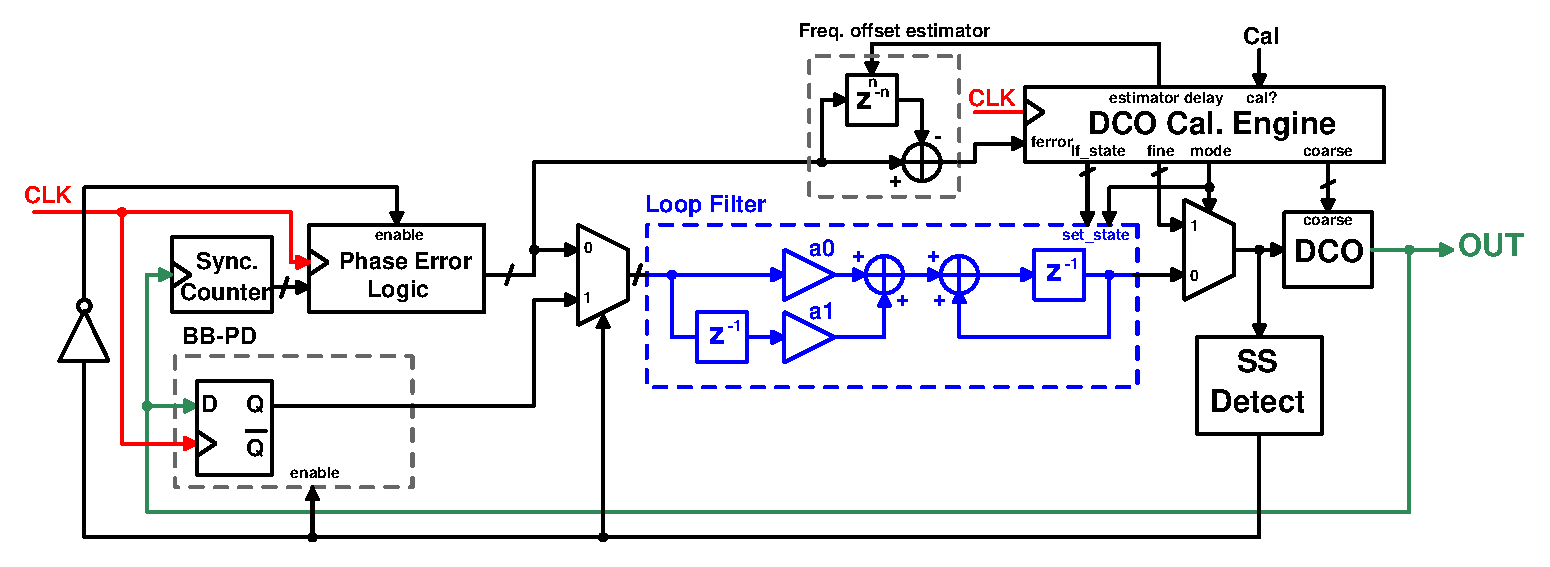
\includegraphics[width=0.8\textwidth, angle=0]{pll_master_arch_28feb2020}

	\end{block}
		\begin{block}{Power Targets {\color{red}(revised)}}
		\scriptsize
		{\color{red}\textbf{(Divider not necessary)}}
		\vspace{-1em}
		\begin{table}[htb!]
			\tiny
			\centering
			\def\arraystretch{1.5}		
			\setlength\arrayrulewidth{0.75pt}
			\setlength{\tabcolsep}{1em} % for the horizontal padding
			\begin{tabular}{|c|c|c|c|c|}
				\hline 
				\rule[-1ex]{0pt}{2.5ex} \cellcolor{gray!40}\textbf{DCO} & \cellcolor{gray!40}\textbf{Phase detector} & \cellcolor{gray!40}\textbf{Digital (LF)}& \cellcolor{gray!40}\textbf{Other} & \cellcolor{gray!40}\textbf{SUM} \\ 
				\hline 
				\rule[-1ex]{0pt}{2.5ex} 50 $\mu$W& 10 $\mu$W &  10 $\mu$W  & \textbf{0} {\color{red}\st{$\leq$ 5}} $ \mu$W & $\leq$ \textbf{70} {\color{red}\st{100}} $\mu$W\\ 
				\hline 
			\end{tabular} 
			% \caption{Assigned specifications for branch line hybrid design.}
			% \label{asgn_specs}
		\end{table}   
	\end{block}

\end{frame}

% #############################################################################
% Specification
% #############################################################################

\begin{frame}
	\frametitle{Specification\color{black}}
	\begin{block}{System Performance Targets}
		\tiny
		\begin{table}[h!]
			\centering
			\def\arraystretch{1.5}		
			\setlength\arrayrulewidth{0.75pt}
			\setlength{\tabcolsep}{1em} % for the horizontal padding
			\begin{tabular}{|l|r|l|l|}
				\hline 
				\rule[-1ex]{0pt}{2.5ex} \cellcolor{gray!40}\textbf{Parameter} & \cellcolor{gray!40}\textbf{Value} & \cellcolor{gray!40}\textbf{Unit }& \cellcolor{gray!40}\textbf{Notes}\\ 
				\hline 
				\rule[-1ex]{0pt}{2.5ex} \textbf{Frequency}  & 2.4-2.4835 & GHz & 2.4G ISM Band\\ 
				\hline 
				\rule[-1ex]{0pt}{2.5ex} \textbf{Ref. frequency} & 16 & MHz & Yields 6 channels \\ 
				\hline 
				\rule[-1ex]{0pt}{2.5ex} \textbf{Power} & $\leq$ \textbf{70} {\color{red}\st{75}} $\mu$W  &$\mu$W & Minimize!\\ 
				\hline 
				\rule[-1ex]{0pt}{2.5ex} \textbf{FSK BER} & $\leq$ 1e-2  & & GFSK\textbf{*} with $f_{dev}$=$\pm$250 KHz\\ 
				\hline 
				\rule[-1ex]{0pt}{2.5ex} \textbf{CNR} & $>$ 20 & dBc&Yields  \textbf{-235} dB FOM$_{jitter}$ ideally \\ 
				\hline 
				\rule[-1ex]{0pt}{2.5ex} \textbf{Initial Lock Time} & $\leq$ 10 & $\mu$s & Upon cold start \\ 
				\hline 
				\rule[-1ex]{0pt}{2.5ex} \textbf{Re-lock Time} & $\leq$ 5 & $\mu$s & Coming out of standby, $f_{error} <$ \textbf{1 MHz} \\ 
				\hline 
				\rule[-1ex]{0pt}{2.5ex} \textbf{Lock $\Delta f$ tolerance} & $100$ & kHz& \\ 
				\hline 
				\rule[-1ex]{0pt}{2.5ex} \textbf{FOM}$_{\textnormal{jitter}}$ & $\leq$ -230 & dB & \textbf{For state of art in size/power} \\ 
				\hline 
				\rule[-1ex]{0pt}{2.5ex} \textbf{Area} & $<$ 0.01  & mm$^2$ & \\ 
				\hline 
			\end{tabular} 
			% \caption{Assigned specifications for branch line hybrid design.}
			% \label{asgn_specs}
		\end{table}   
		\textbf{*} Using BT=0.3, 1 MSymbols/s, 4 demodulated symbols averaged per bit to yield 250 kbps.
	\end{block}    
\end{frame}



\begin{frame}
	\frametitle{Specification\color{black}}
	\begin{block}{Component-level specs}
		\scriptsize
	\begin{table}[h!]
		\centering
		\tiny
		\def\arraystretch{1.5}		
		\setlength\arrayrulewidth{0.75pt}
		\setlength{\tabcolsep}{1em} % for the horizontal padding
		\begin{tabular}{|l|r|l|}
			\hline 
			\rule[-1ex]{0pt}{2.5ex} \cellcolor{gray!40}\textbf{Parameter} & \cellcolor{gray!40}\textbf{Value} & \cellcolor{gray!40}\textbf{Unit }\\ 
			\hline 
			\rule[-1ex]{0pt}{2.5ex} \textbf{Counter range}  & 256 steps & coverage of 150-155 \\ 
			\hline 
			\rule[-1ex]{0pt}{2.5ex} \textbf{Divider ratio} & 150-155  & (For non-counter based)\\ 
			\hline 
			\rule[-1ex]{0pt}{2.5ex} {\color{red}\st{\textbf{TDC resolution}}} &{\color{red}\st{$\geq$ 155}}  & {\color{red}\st{steps/reference cycle}}\\ 
			\hline 
			\rule[-1ex]{0pt}{2.5ex} \textbf{DCO gain $K_{DCO}$} & $10^4$ & Hz/LSB \\ 
			\hline 
			\rule[-1ex]{0pt}{2.5ex} \textbf{DCO tuning range} & 10 & MHz \\ 
			\hline 
			\rule[-1ex]{0pt}{2.5ex} \textbf{DCO DAC resolution} & 10 & bit \\ 
			\hline 
			\rule[-1ex]{0pt}{2.5ex} \textbf{DCO Phase noise} &$<$ -80 & dBc/Hz @ $\Delta f=10^6$ Hz, $f_c$ = 2.448 GHz \\ 
			\hline 
			\rule[-1ex]{0pt}{2.5ex} \textbf{DCO Power} & $\leq$ 50 & $\mu$W \\ 
			\hline 
			\rule[-1ex]{0pt}{2.5ex} \textbf{Digital filter word resolution} & $\leq$ 16 & bits (power grows as $\mathcal{O}(n^2)$) \\ 
			\hline 
			\rule[-1ex]{0pt}{2.5ex} \textbf{BB-PD jitter} & $\leq$ 12 & ps$_{\textnormal{rms}}$ \\ 
			\hline 
		\end{tabular} 
		% \caption{Assigned specifications for branch line hybrid design.}
		% \label{asgn_specs}
		\label{design_specs}
	\end{table}   
	\end{block}    
\end{frame}

% #############################################################################
% Timeline
% #############################################################################

\begin{frame}
	\frametitle{Time plan (pt. 1)}
	\begin{table}[htb!]
		\tiny
		\centering
		\vspace{-1em}
		\def\arraystretch{1.5}		
		\setlength\arrayrulewidth{0.75pt}
		\setlength{\tabcolsep}{1em} % for the horizontal padding
		\begin{tabular}{|c|l|l|l|}
			\hline 
			\rule[-1ex]{0pt}{2.5ex}\cellcolor{gray!40}\textbf{Week \#} & \cellcolor{gray!40}\textbf{Dates} &\cellcolor{gray!40}\textbf{Tasks} & \cellcolor{gray!40}\textbf{Outcomes}\\ 
			\hline 
			% \rule[-1ex]{0pt}{2.5ex} \cellcolor{green!20}\textbf{3}&\cellcolor{green!20}13.1 - 19.1 &\cellcolor{green!20}Review PLL Design &\cellcolor{green!20}Refreshed Knowledge\\ 
			% \hline 
			\rule[-1ex]{0pt}{2.5ex}\cellcolor{red!40}\textbf{4}&\cellcolor{red!40}20.1 - 26.1 &\cellcolor{red!40}Finalize high level modeling &\cellcolor{red!40}Component level specification\\ 
			\hline 
			\rule[-1ex]{0pt}{2.5ex}\textbf{5}\cellcolor{red!40}&\cellcolor{red!40}27.1 - 2.2 &\cellcolor{red!40}Establish test bench in Virtuoso &\cellcolor{red!40}With ideal PLL implementation\\ 
			\hline 
			\rule[-1ex]{0pt}{2.5ex}\cellcolor{red!40}\textbf{6}&\cellcolor{red!40}3.2 - 9.2&\cellcolor{red!40}Schem. design: phase detector &\cellcolor{red!40}TDC - flash and counter based \\ 
			\hline 
			\rule[-1ex]{0pt}{2.5ex}\cellcolor{red!40}\textbf{7}&\cellcolor{red!40}10.2 - 16.2&\cellcolor{red!40}Schem. design: phase detector &\cellcolor{red!40}Bang-bang phase detector\\ 
			\hline 
			\rule[-1ex]{0pt}{2.5ex}\cellcolor{red!40}\textbf{8}&\cellcolor{red!40}17.2 - 23.2&\cellcolor{red!40}RTL, synthesis, place\&route &\cellcolor{red!40}Digital loop filter\\ 
			\hline 
			\rule[-1ex]{0pt}{2.5ex}\cellcolor{red!40}\textbf{9}&\cellcolor{red!40}24.2 - 1.3&\cellcolor{red!40}RTL, synthesis, place\&\cellcolor{red!40}route & \cellcolor{red!40}Digital loop filter\\ 
			\hline 
			\rule[-1ex]{0pt}{2.5ex}\cellcolor{red!40}\textbf{10}&\cellcolor{red!40}2.3 - 8.3&\cellcolor{red!40}Schem. design: oscillator &\cellcolor{red!40}Ring DCO\\ 
			\hline 
			\rule[-1ex]{0pt}{2.5ex}\cellcolor{red!40}\textbf{11}&\cellcolor{red!40}9.3 - 15.3&\cellcolor{red!40}Layout: oscillator &\cellcolor{red!40} \\ 
			\hline 
			\rule[-1ex]{0pt}{2.5ex}\cellcolor{green!40}\textbf{12}&\cellcolor{green!40}16.3 - 22.3&\cellcolor{green!40}CDAC/Ring oscillator  &\cellcolor{green!40}Layout\\ 
			\hline 
			\rule[-1ex]{0pt}{2.5ex}\textbf{13}&23.3 - 29.3&CDAC/Ring oscillator   & Layout\\ 
			\hline 
			\rule[-1ex]{0pt}{2.5ex}\textbf{14}& 30.3 - 5.4 &  Calibration/control logic & RTL, synth, PnR for calibration\\ 
			\hline 
			\rule[-1ex]{0pt}{2.5ex}\textbf{15}& 6.4 - 12.4& {\color{red}\textbf{Easter}} & - \\ 
			\hline 
			\rule[-1ex]{0pt}{2.5ex}\textbf{16}& 13.4 - 19.4& Layout & Phase detector\\ 
			\hline 
			\rule[-1ex]{0pt}{2.5ex}\textbf{17}& 20.4 - 26.4& Layout & Oscillator\\ 
			\hline 
		\end{tabular}
		\begin{flushleft}\textbf{Legend:} \colorbox{red!20}{\textbf{Done}} \colorbox{green!20}{\textbf{Current}}  \colorbox{blue!20}{\textbf{Revised}}
		% *I will write the report simultaneously with the work.
		\end{flushleft}
		% \caption{Assigned specifications for branch line hybrid design.}
		% \label{asgn_specs}
	\end{table}   
\end{frame}

\begin{frame}
	\frametitle{Time plan (pt. 2)}
	\begin{table}[htb!]
		\tiny
		\centering
		\vspace{-1em}
		\def\arraystretch{1.5}		
		\setlength\arrayrulewidth{0.75pt}
		\setlength{\tabcolsep}{1em} % for the horizontal padding
		\begin{tabular}{|c|l|l|l|}
			\hline 
			\rule[-1ex]{0pt}{2.5ex}\cellcolor{gray!40}\textbf{Week \#} & \cellcolor{gray!40}\textbf{Dates} &\cellcolor{gray!40}\textbf{Tasks} & \cellcolor{gray!40}\textbf{Outcomes}\\ 
			\hline 
			\rule[-1ex]{0pt}{2.5ex}\textbf{18}& 27.4 - 3.5 & Layout & Divider/calibration\\ 
			\hline 
			\rule[-1ex]{0pt}{2.5ex}\textbf{19}& 4.5 - 10.5 & Layout & Finalization/system integration\\ 
			\hline 
			\rule[-1ex]{0pt}{2.5ex}\textbf{20}& 11.5 - 17.5 & Flex week (layout) OR yield improvement & Depending on progress\\ 
			\hline 
			\rule[-1ex]{0pt}{2.5ex}\textbf{21}& 18.5 - 24.5& {\color{blue}\textbf{Report writing}} & \\ 
			\hline 
			\rule[-1ex]{0pt}{2.5ex}\textbf{22}& 25.5 - 31.5& {\color{blue}\textbf{Report writing}} & \\ 
			\hline 
			\rule[-1ex]{0pt}{2.5ex}\textbf{23}& 1.6 - 7.6& {\color{blue}\textbf{Report writing}} & {\color{red}\textbf{Deadline 8.6}}\\ 
			\hline 
		\end{tabular}
		\begin{flushleft}\textbf{Legend:} \colorbox{red!20}{\textbf{Done}} \colorbox{green!20}{\textbf{Current}}  \colorbox{blue!20}{\textbf{Revised}}
		% *I will write the report simultaneously with the work.
		\end{flushleft}
		% \caption{Assigned specifications for branch line hybrid design.}
		% \label{asgn_specs}
	\end{table}   
\end{frame}


% #############################################################################
% project phases
% #############################################################################

% ############################################################################b#
% References
% #############################################################################


\begin{frame}
	\frametitle{References}
		\scriptsize
		[1] L. Dai and R. Harjani, "Analysis and design of low-phase-noise ring oscillators," ISLPED'00: Proceedings of the 2000 International Symposium on Low Power Electronics and Design (Cat. No.00TH8514), Rapallo, Italy, 2000, pp. 289-294. doi: 10.1145/344166.344639\par
		\vspace{0.5em}
		[2] A. Hajimiri and T. H. Lee, "A general theory of phase noise in electrical oscillators," in IEEE Journal of Solid-State Circuits, vol. 33, no. 2, pp. 179-194, Feb. 1998.\par
		% [1]  Liu, H., Shirane, A., Okada, K., Sun, Z., Huang, H., Deng, W., Siriburanon, T., Pang, J., Wang, Y., Wu, R. and Someya, T. (2019). A 265-$\mu$ W Fractional-${N}$ Digital PLL With Seamless Automatic Switching Sub-Sampling/Sampling Feedback Path and Duty-Cycled Frequency-Locked Loop in 65-nm CMOS. IEEE Journal of Solid-State Circuits, 54(12), pp.3478-3492.
		\vspace{0.5em}
		[3] G. Jacquemod et al., "Study and reduction of variability in 28 nm FDSOI technology," 2015 International Workshop on CMOS Variability (VARI), Salvador, 2015, pp. 19-22.\par
		\vspace{0.5em}

		% [1]  H. Xu and A. A. Abidi, “Design Methodology for Phase-Locked Loops Using Binary (Bang-Bang) Phase Detectors,” IEEE Transactions on Circuits and Systems I: Regular Papers, vol. 64, no. 7, pp. 1637–1650, Jul. 2017.\par
		% \vspace{0.5em}
		% [2] F. Gardner, “Charge-Pump Phase-Lock Loops,” IEEE Transactions on Communications, vol. 28, no. 11, pp. 1849–1858, Nov. 1980, doi: 10.1109/tcom.1980.1094619.\par
		% \vspace{0.5em}
		% [3] Liu, B., Li, Z., Fu, X., Shirane, A., Kurosu, H., Nakane, Y., Masaki, S., Okada, K., Zhang, Y., Qiu, J., Huang, H., Sun, Z., Xu, D., Zhang, H., Wang, Y. and Pang, J. (2020). A Fully-Synthesizable Fractional-N Injection-Locked PLL for Digital Clocking with Triangle/Sawtooth Spread-Spectrum Modulation Capability in 5 nm CMOS. IEEE Solid-State Circuits Letters, pp.1-1.
	% Navid et al. 2005
\end{frame}


\end{document}
